% \newgeometry{margin = 1in , top = 0in}
% \voffset=-0.in
\chapter{Problem Statement}
% \titleformat{\section}{\large\bfseries}{\thesection}{1em}{\ }
\section{Indian Railways}
\pagenumbering{arabic}\hspace{3mm}

Let us first describe the nature of the railway system in this country. 
The Indian railway network is designed to consist of long ‘lines’ (a string of stations),
which connect with each other at ‘junction’ stations. Each station is composed 
of one or more parallel \textbf{tracks}, which may be associated with a fixed direction of 
traffic, or they could be bidirectional. Similarly, there are one or more tracks 
between each neighbouring pair of stations. These tracks are typically referred 
to as \textbf{sections}, in order to differentiate them from tracks actually at a station. 
The section tracks can also be unidirectional (fixed direction of train movement)
 or bidirectional. The Indian network typically consists of sections with one or two tracks. 
\\
\\
 \begin{figure}[H]
    \centering
    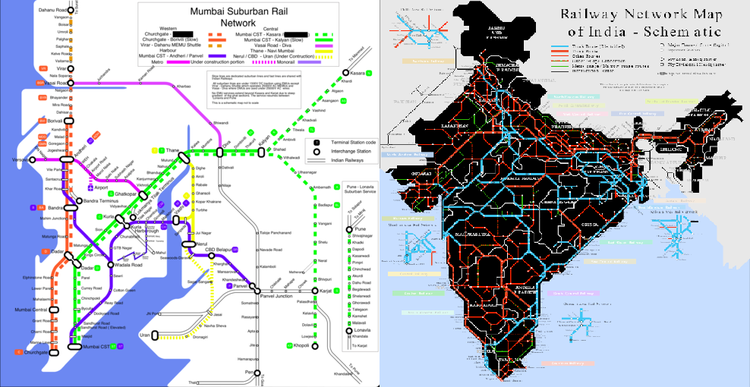
\includegraphics[width=0.8\textwidth]{Railways_pic}
    \caption{The line and junction topology of railway networks in India \cite{WEBSITE:1}. }
    \label{image-myimage}
\end{figure}

The approach we are focussing on now deals with linear railway 
networks with multiple parallel tracks, of the type shown in figure 2.2. This
restriction on topology is reasonable because rail networks are
designed in the form of multi-station linear arcs connected
at junction stations.

\begin{figure}[H]
    \centering
    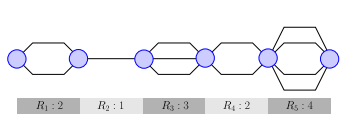
\includegraphics[width=0.4\textwidth]{report1}
    \caption{Linear Railway Lines \cite{ARTICLE:1}. }
    \label{image-myimage}
\end{figure}

\section{Railway Scheduling Problem}
\subsection{Scheduling}
A specific problem instance begins by defining the resources
on the railway line, as given by the number of stations, their
order, and the number of parallel tracks (both at each station
and between two neighbouring stations). Besides resource level information, 
train movements over the scheduling horizon must be described in one of two ways.
\begin{itemize}
    \item To define a reference timetable which gives the desired arrival
    and departure time of each train at each station.
    \item To provide the earliest movement times from their
    current locations (or origin stations), followed by the minimum
    running times (on track sections between stations) and halt
    times (at stations) up to the destinations.
\end{itemize}

\vspace{0.2cm}

Note that the running
and halt times can be completely heterogeneous: each train
may have a different running/halt time in each resource,
depending on the length of track, the type of halt, and the
type of locomotive.

\vspace{0.2cm}
Timetabling refers to an offline planning problem for a railway network.
\textbf{Given a set of trains and their origins and destinations (with or without a fixed route),
 the goal is to assign track resources for each train for a fixed time period, 
 such that they all complete their journeys without conflicts.}

 \vspace{0.2cm}
 Such a timetable may be infeasible if the desired arrival and
departure times violate the track usage rules defined earlier.
The task of the scheduling algorithm is to adjust the arrival
and departure times such that all rules are satisfied, while
minimizing an objective called priority-weighted delay. This schedule
is to be computed for all trains up to their destinations.

\vspace{0.2cm}
The railway problem has been shown in literature to be a \textbf{‘blocking’ version of the 
Job Shop Scheduling Problem (JSSP)}, where the job (train) must wait in the current resource 
(track) until the next resource is freed (there is no buffer for storing jobs between 
two resources). This version of the JSSP is also \textbf{NP complete}, with the result that 
exact solutions require an exponential amount of time for computation.
\vspace{1in}
\subsection{Rescheduling}

Another problem is that of rescheduling.
Rescheduling is the online counterpart of the timetabling problem , 
where the goal is to recover from a disruption to the timetable, 
caused by delays or faults. The mathematical differences are found in two aspects. 
\begin{itemize}
\item The goal is to return to the original timetable using built-in slack times, 
instead of defining the timetable itself. 
This implies that the objective function would focus on minimizing delays to 
trains with respect to the timetable, or the time required for deviations to the smoothed out. 
\item The online nature of the problem implies that there is very limited time 
available to compute solutions, and that sub-optimal but reasonably efficient 
solutions are acceptable. 
\end{itemize}

% \section{Time Table Scheduling problem}

